\section{Illumination models}
The goal of an illumination model is to quantify the amount of reflected light on a surface that is captured by a camera. An illumination model depends on three factors:

\begin{enumerate}
    \item Light source parameters: position, intensity, electromagnetic spectrum;
    \item Surface parameters (material): position, shape, reflectance properties;
    \item Camera parameters: position, sensor spectrum sensitivity.
\end{enumerate}

The illumination model defines the mathematical calculation that will be used to define the light reflected off a specific point on the surface of an object in a specific direction.

\section{Shading models}
A shading model is a rendering method which will apply an illumination model to determine the light intensity in all pixels of the image. Defines how the illumination model is used to render a shaded image. The most popular shading models are flat, Gouraud and Phong shading, shown in Figure \ref{fig:shading_models}.

\begin{figure}[h]
    \begin{center}
        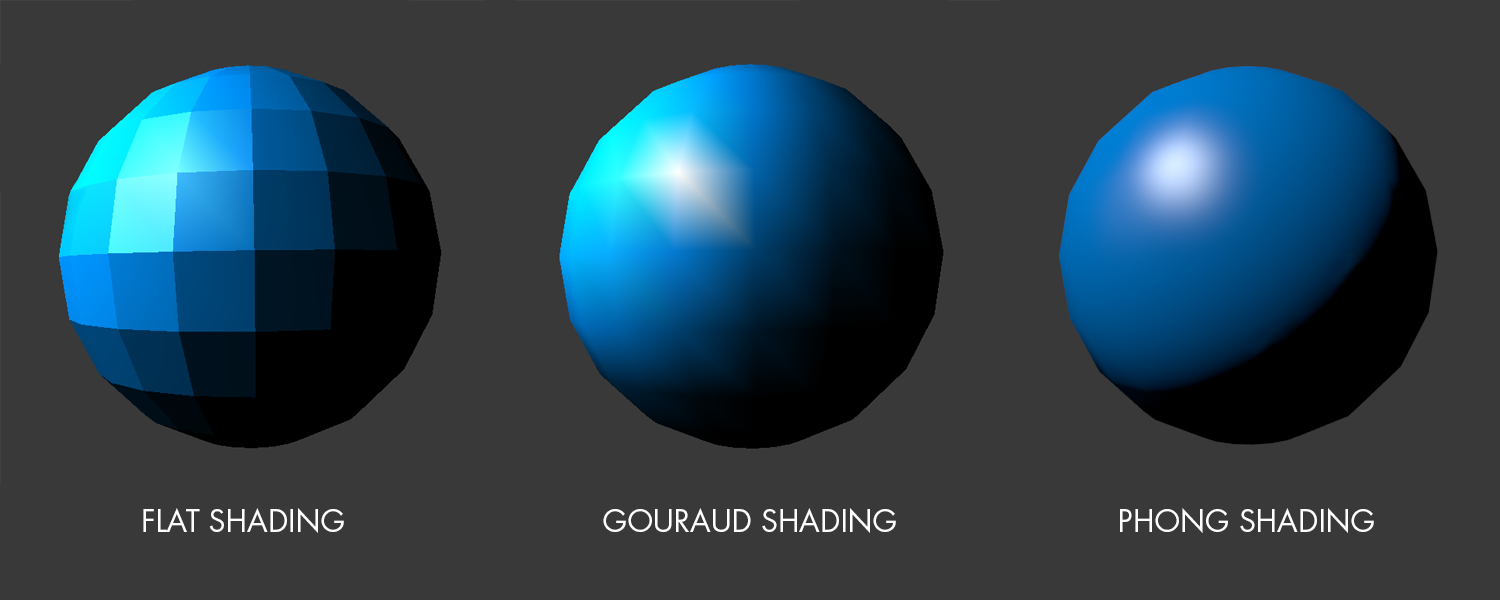
\includegraphics[width = 15cm]{figs/shading_models.png}
    \end{center}
    \caption{Popular shading models}
    \label{fig:shading_models}
\end{figure}

\section{Shading languages}
Shading languages are programming languages designed for computer graphics, which are used to write shader programs, implementing an illumination model. Various shading languages exist:

\begin{itemize}
    \item CG: \emph{C for Graphics}, developed by NVidia in collaboration with Microsoft, it has been deprecated since 2012;
    \item HLSL: \emph{High-Level Shader Language}, used with DirectX 9 and higher;
    \item GLSL: \emph{OpenGL Shading Language}, used with OpenGL.
\end{itemize}

In this work, all the shader code was written in GLSL. We will not be covering the GLSL language specifics, as it goes beyond the scope of this text.
